\documentclass{article}
\usepackage{graphicx}

\title{Comparison between AVL and BST trees }
\author{Giray Sahin}

\begin{document}
\maketitle
\section{Introduction}
Our target is implementing a Binary Search Tree and an AVL tree that hold strings, and comparing insterion and search times.



\subsection{AVL trees}
AVL is a consistently balenced binary search tree. We provide the equivalency by checking the depth of nodes. 

The balancing factor of a node is the difference between the heights of its left and right subtrees. A balancing factor of -1, 0, or 1 indicates a balanced tree, while any other value triggers the rotation operations.

Assuming AVL tree, the height of the subtrees(childs) of any node differences can be maximum 1 or 0. That ensures that the tree remains balanced. Provide that we have to keep the tree balanced during the instertion and deletion operations. 

This self-balancing property ensures efficient search, insertion, and deletion operations with a worst-case time complexity of O(log(n)), where n is the number of nodes in the tree.

\subsection{Binary search trees}

    A Binary Search Tree (BST) is a data structure where each node has at most 2 child nodes, and the data in the nodes follow a small-size relationship. The left branch of each node contains data less than the node's value, and the right branch contains data greater than the node's value. 

This organization enables an efficient binary search algorithm, with a time complexity of O(log n) for search, insertion, and deletion operations, where 'n' is the number of nodes. Certain variants, like AVL trees, introduce a self-balancing feature to maintain efficiency during dynamic data modifications by using balancing factors and rotations. 

However, it's important to note that while AVL trees offer efficient operations, they come with a slight overhead in terms of additional storage and computational requirements. In real-world applications, binary search trees, including AVL trees, find utility in scenarios where ordered data storage and retrieval are crucial, such as in databases for indexing and efficient data retrieval.

\maketitle
\section{Methodology}
TDK the Turkish Language Institute has a website with a dictionary but it doesn't have an api so we had to scrape it. And then we sorted the random data using a custom sorting key based on the Turkish alphabet order. 
Implemented a Binary Search Tree (BST) and an AVL Tree from scratch in C++. And we ensured consistency in the programming language throughout the implementation. And then we compared the instersion and search times.
We can also change the insertion size and check the comparison times with large data sizes.


\maketitle
\section{Results}
Based on the results in the results.txt file, we can draw the following conclusions, with the input size of 10000:\\\\
Random Data: Both Binary Search Tree (BST) and AVL tree perform well with random data. However, BST has a slightly better performance in insertion time (9 ms vs 7 ms), while AVL tree has a better performance in search time (10 ms vs 5 ms).\\\\
Ordered Data: AVL tree performs significantly better than BST with ordered data. BST has a much higher insertion and search time (178 ms and 127 ms respectively) compared to AVL tree (both 8 ms and 4 ms respectively). This is because BSTs can become unbalanced with ordered data, turning into a linked list with O(n) search time. AVL trees, on the other hand, maintain balance and thus have a much faster insertion and search time.\\\\
Nearly Ordered Data: AVL trees also perform better with nearly ordered data. BST has insertion and search times of 36 ms and 35 ms respectively, while AVL tree has insertion and search times of 11 ms and 4 ms respectively.\\\\
\newpage
\begin{figure}[h]
\centering
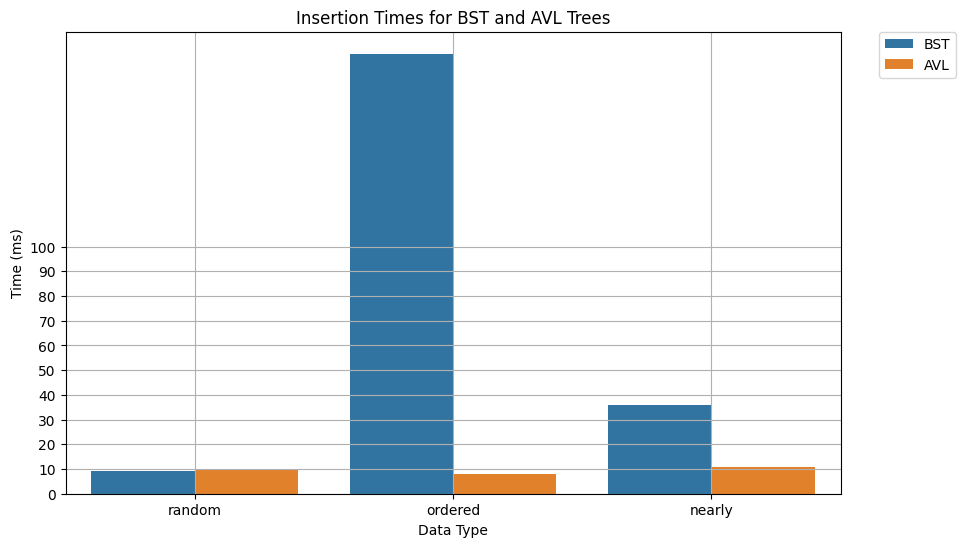
\includegraphics[width=0.9\textwidth]{../data/graphs/insertion_times.png}
\caption{Insertion times comparison}
\end{figure}


\begin{figure}[h]
\centering
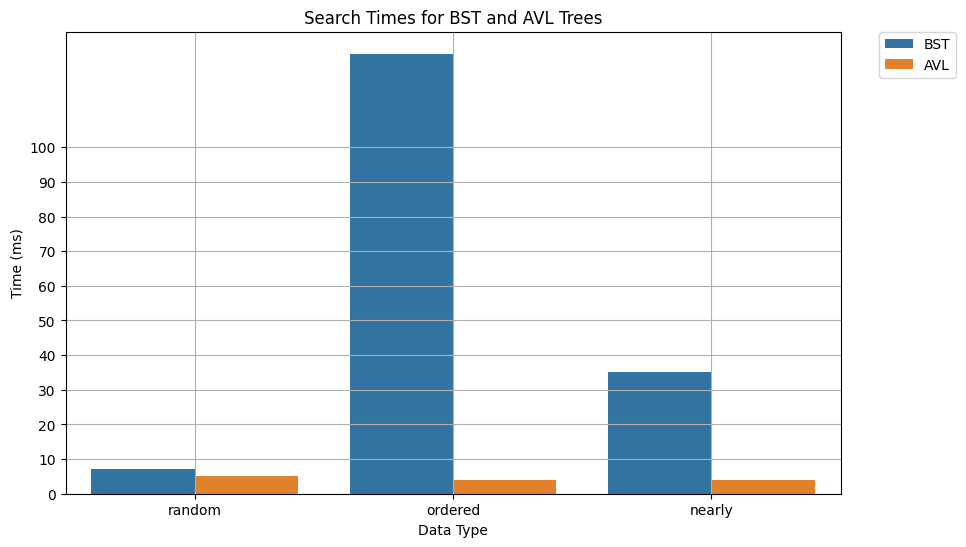
\includegraphics[width=0.9\textwidth]{../data/graphs/search_times.png}
\caption{Search times comparison}
\end{figure}
\newpage


\maketitle
\section{Conclusions}

In conclusion, while BSTs can perform slightly better with random data, AVL trees are generally more reliable and performant with both ordered and nearly ordered data due to their self-balancing properties.


\end{document}